\documentclass{article}
\usepackage[T2A]{fontenc}
\usepackage[utf8]{inputenc}
\usepackage[russian]{babel}
\usepackage{def_style}
\usepackage[hyper]{amsbib}
\usepackage{wrapfig}
\usepackage{multicol}
\usepackage{blindtext}
\usepackage{multirow}
\usepackage{cellspace, longtable}
\setlength\cellspacetoplimit{3pt}
\setlength\cellspacebottomlimit{3pt}
\usepackage{booktabs}
% Verbatim words:
\usepackage{fancyvrb}
\DeclareMathSymbol{\shortminus}{\mathbin}{AMSa}{"39}
\usepackage{listings}
\lstdefinestyle{mystyle}{
    keywordstyle=\color{blue},              
    basicstyle=\ttfamily\normalsize,
    columns=fullflexible,
    keepspaces=true,
    commentstyle=\color{codegreen}
}
\lstdefinestyle{inline_style}{
	language={[LaTeX]TeX},
    basicstyle=\ttfamily\Large\bfseries
}
\lstset{style=mystyle}
% Title settings:
\usepackage{titlesec}
\titleformat{\section}
  {\normalfont\Large\bfseries}{\thesection.}{1em}{}
% Numbering settings:
%\renewcommand{\theequation}{\thesection.\arabic{equation}}
%\counterwithin*{equation}{section}
% Theorem settings:
\theoremstyle{definition}
\newtheorem*{definition}{Определение}
\newtheorem*{theorem}{Теорема}
\newtheorem*{statement}{Теорема}
\newtheorem{task}{Задание}
% Specific commands:
\newcommand{\ExternalLink}{%
\tikz[x=1.2ex, y=1.2ex, baseline=-0.05ex]{% 
    \begin{scope}[x=1ex, y=1ex]
        \clip (-0.1,-0.1) 
            --++ (-0, 1.2) 
            --++ (0.6, 0) 
            --++ (0, -0.6) 
            --++ (0.6, 0) 
            --++ (0, -1);
        \path[draw, 
            line width = 0.5, 
            rounded corners=0.5] 
            (0,0) rectangle (1,1);
    \end{scope}
    \path[draw, line width = 0.5] (0.5, 0.5) 
        -- (1, 1);
    \path[draw, line width = 0.5] (0.6, 1) 
        -- (1, 1) -- (1, 0.6);
    }
}
\usepackage[labelsep=period]{caption}
\usepackage{csquotes}
\usepackage{subcaption}
\newcommand{\q}[1]{``#1''}
\title{\textbf{Аппроксимация конформных отображений}}
\author{Скажите, пожалуйста, - вежливо начала Алиса, - как и куда вы \\
\textbf{конформно отображаете} эти чудесные \textbf{розы}?}
\date{Ознакомительная практика ФН1-41Б --- \today}
\begin{document}
\maketitle
Аппарат теории конформных отображений является незаменимым инструментом в арсенале современных математиков и детально описан на страницах многих учебников, справочников и каталогов (см., например, \cite{1}\cite{2}\cite{3}). Традиционно в теории и практике конформных отображений  выделяются следующие два основных направления:
\begin{itemize}
\item[---] \textit{прямая} задача нахождения образа некоторой кривой или области при заданном отображении, которой и будет посвящена данная практика;
\item[---] \textit{обратная} (и крайне нетривиальная) задача нахождения функции, реализующей конформное отображение между двумя заданными областями. Особо любопытным студентам, которых скорее всего не устраивает наша мимолётная и крайне субъективная ремарка о сложности таких задач, осмелимся лишь предложить попробовать конформно отобразить прямоугольник на верхнюю полуплоскость.
\end{itemize}
\section{Численное отображение областей}
Напомним классический результат из теории функций комплексного переменного \cite{Shabat}:
\begin{theorem}[Принцип соответствия границ Каратеодори] 
Пусть области $D$ и $D'$ ограничены \textit{жордановыми кривыми} $\partial D$ и $\partial D'$; тогда конформное отображение $f:D\rightarrow D'$ можно продолжить на границу $D$ до гомеоморфизма замкнутых областей $\overline{D}$ и $\overline{D'}$.
\end{theorem} \noindent
Таким образом, оперируя в рамках этой теоремы и предполагая что искомый образ $D'$ также ограничен жордановой кривой $\partial D'$, нахождение образа некоторой области $D$ можно свести \textit{к нахождению образа её границы} $\partial D$. Если же нам известна и некоторая \textit{параметризация} $g:T\rightarrow \partial D$ границы исходной области, то можно использовать довольно простой и эффективный алгоритм \textbf{A1.1} построения $\partial D'$ (см. рис. 1). \vspace*{-0.4cm}
\begin{figure}[h!]
    \centering
    \hspace{-0.5cm}
    \begin{subfigure}{0.48\textwidth}
        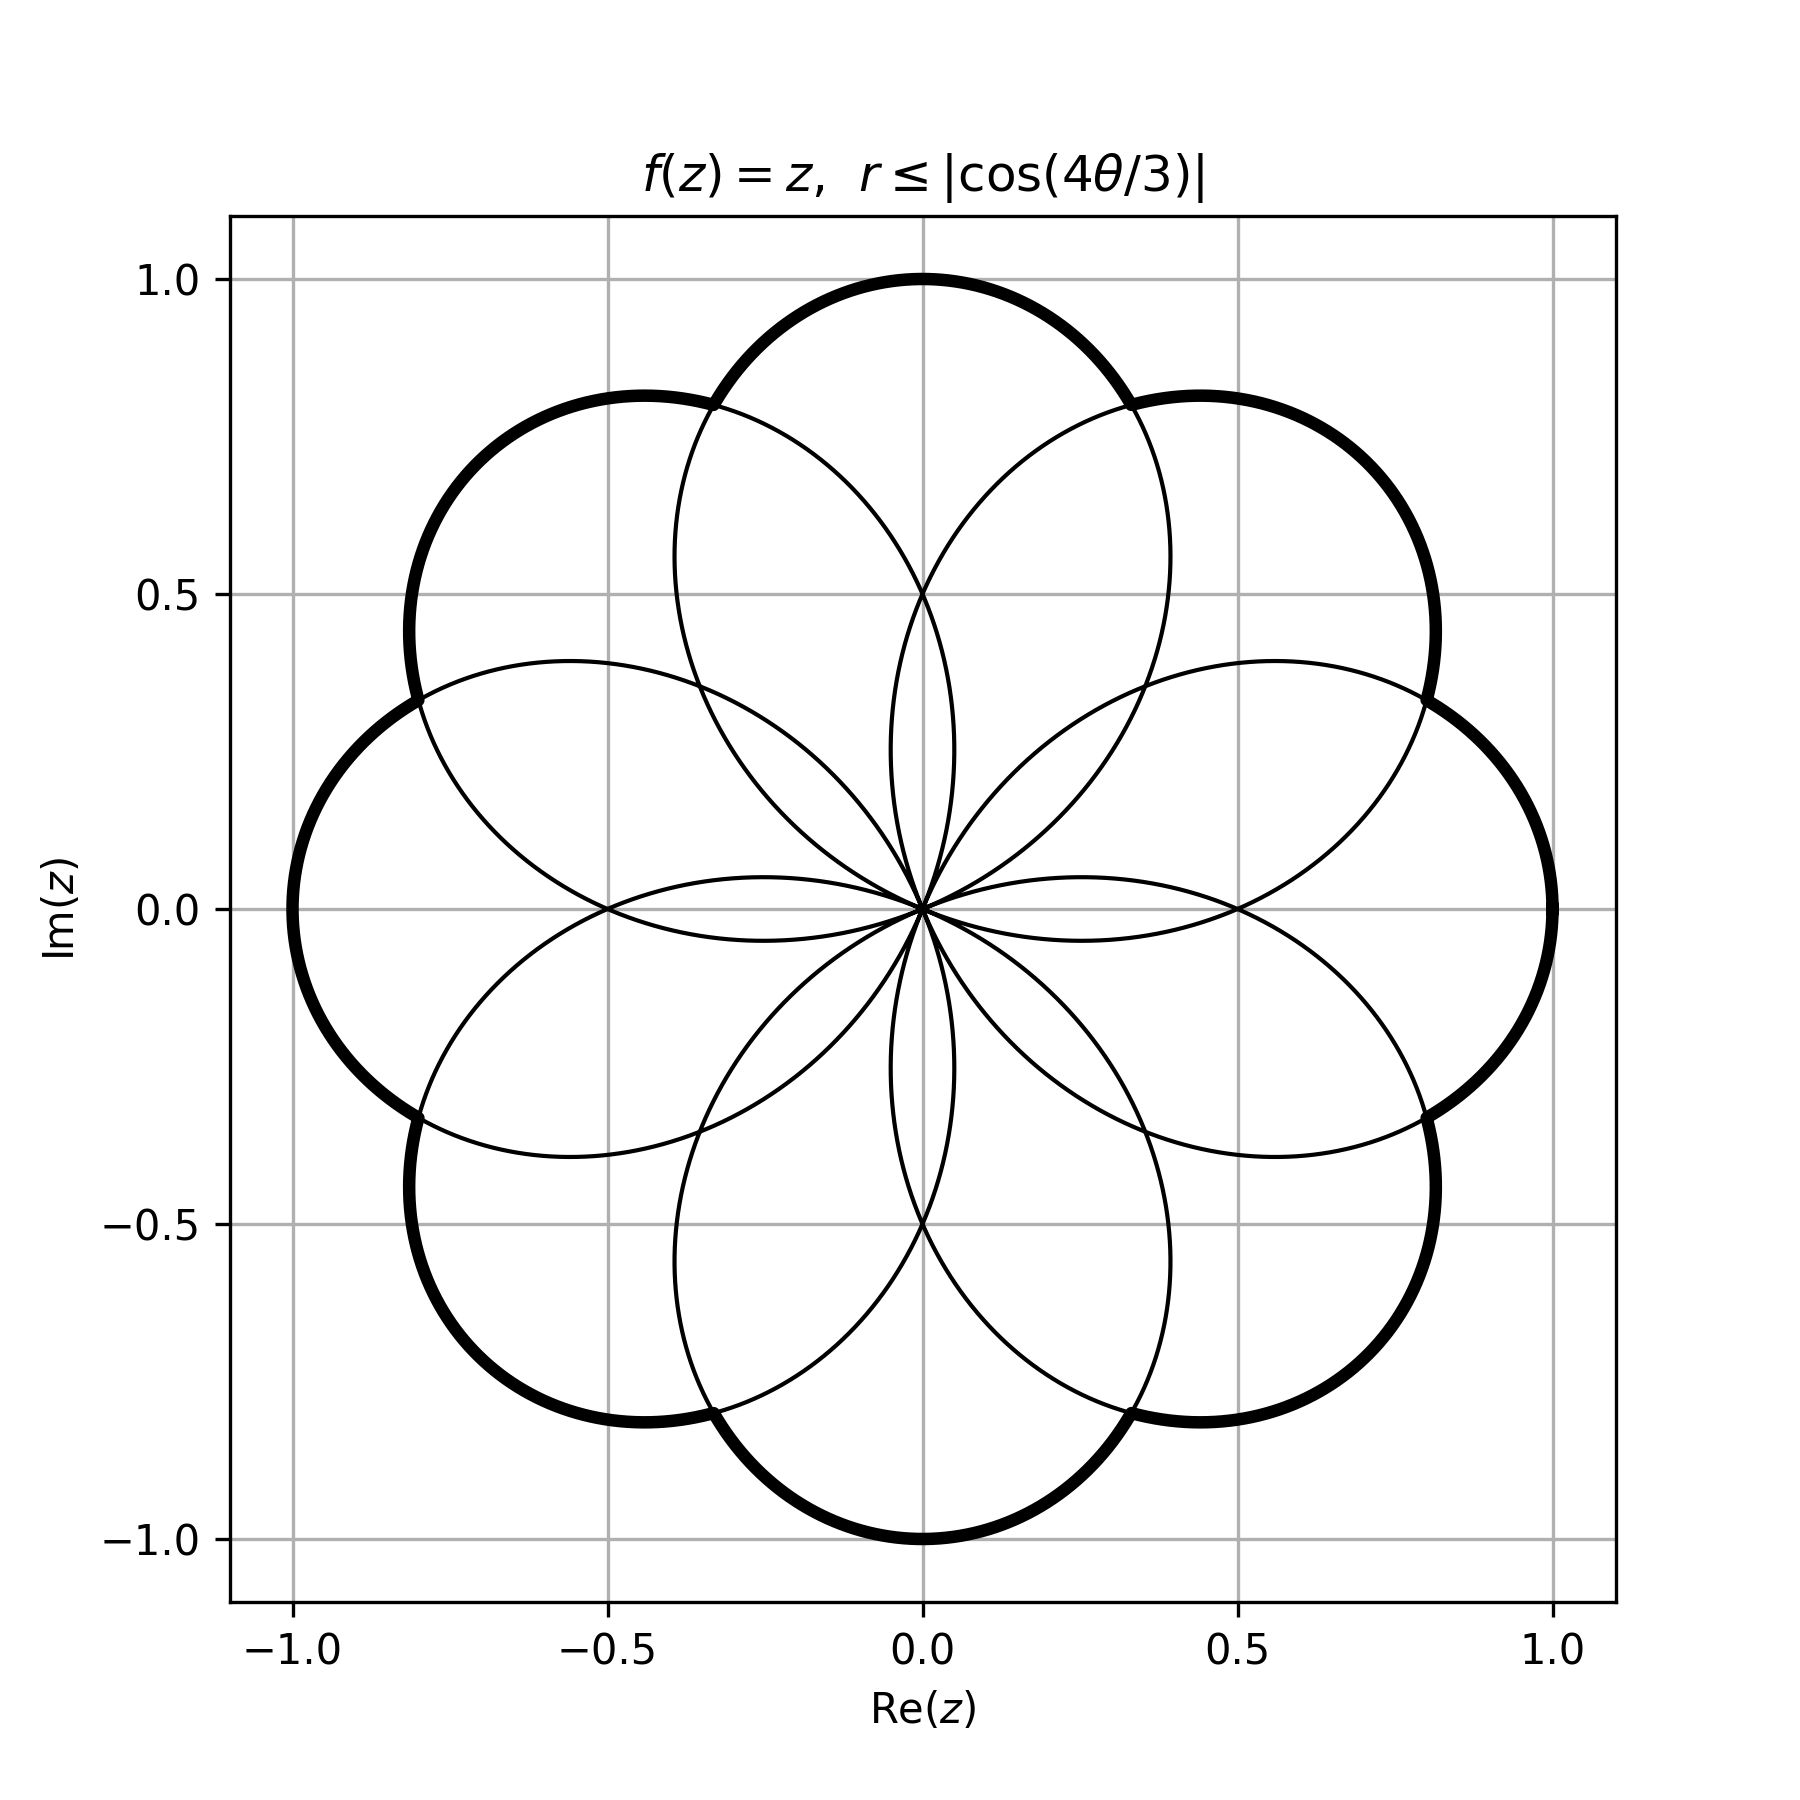
\includegraphics[width=\textwidth]{img/init_flower300dpi.png}
        \caption{\; Прообраз розы}
    \end{subfigure} \hspace{0.1cm}
    \begin{subfigure}{0.48\textwidth}
        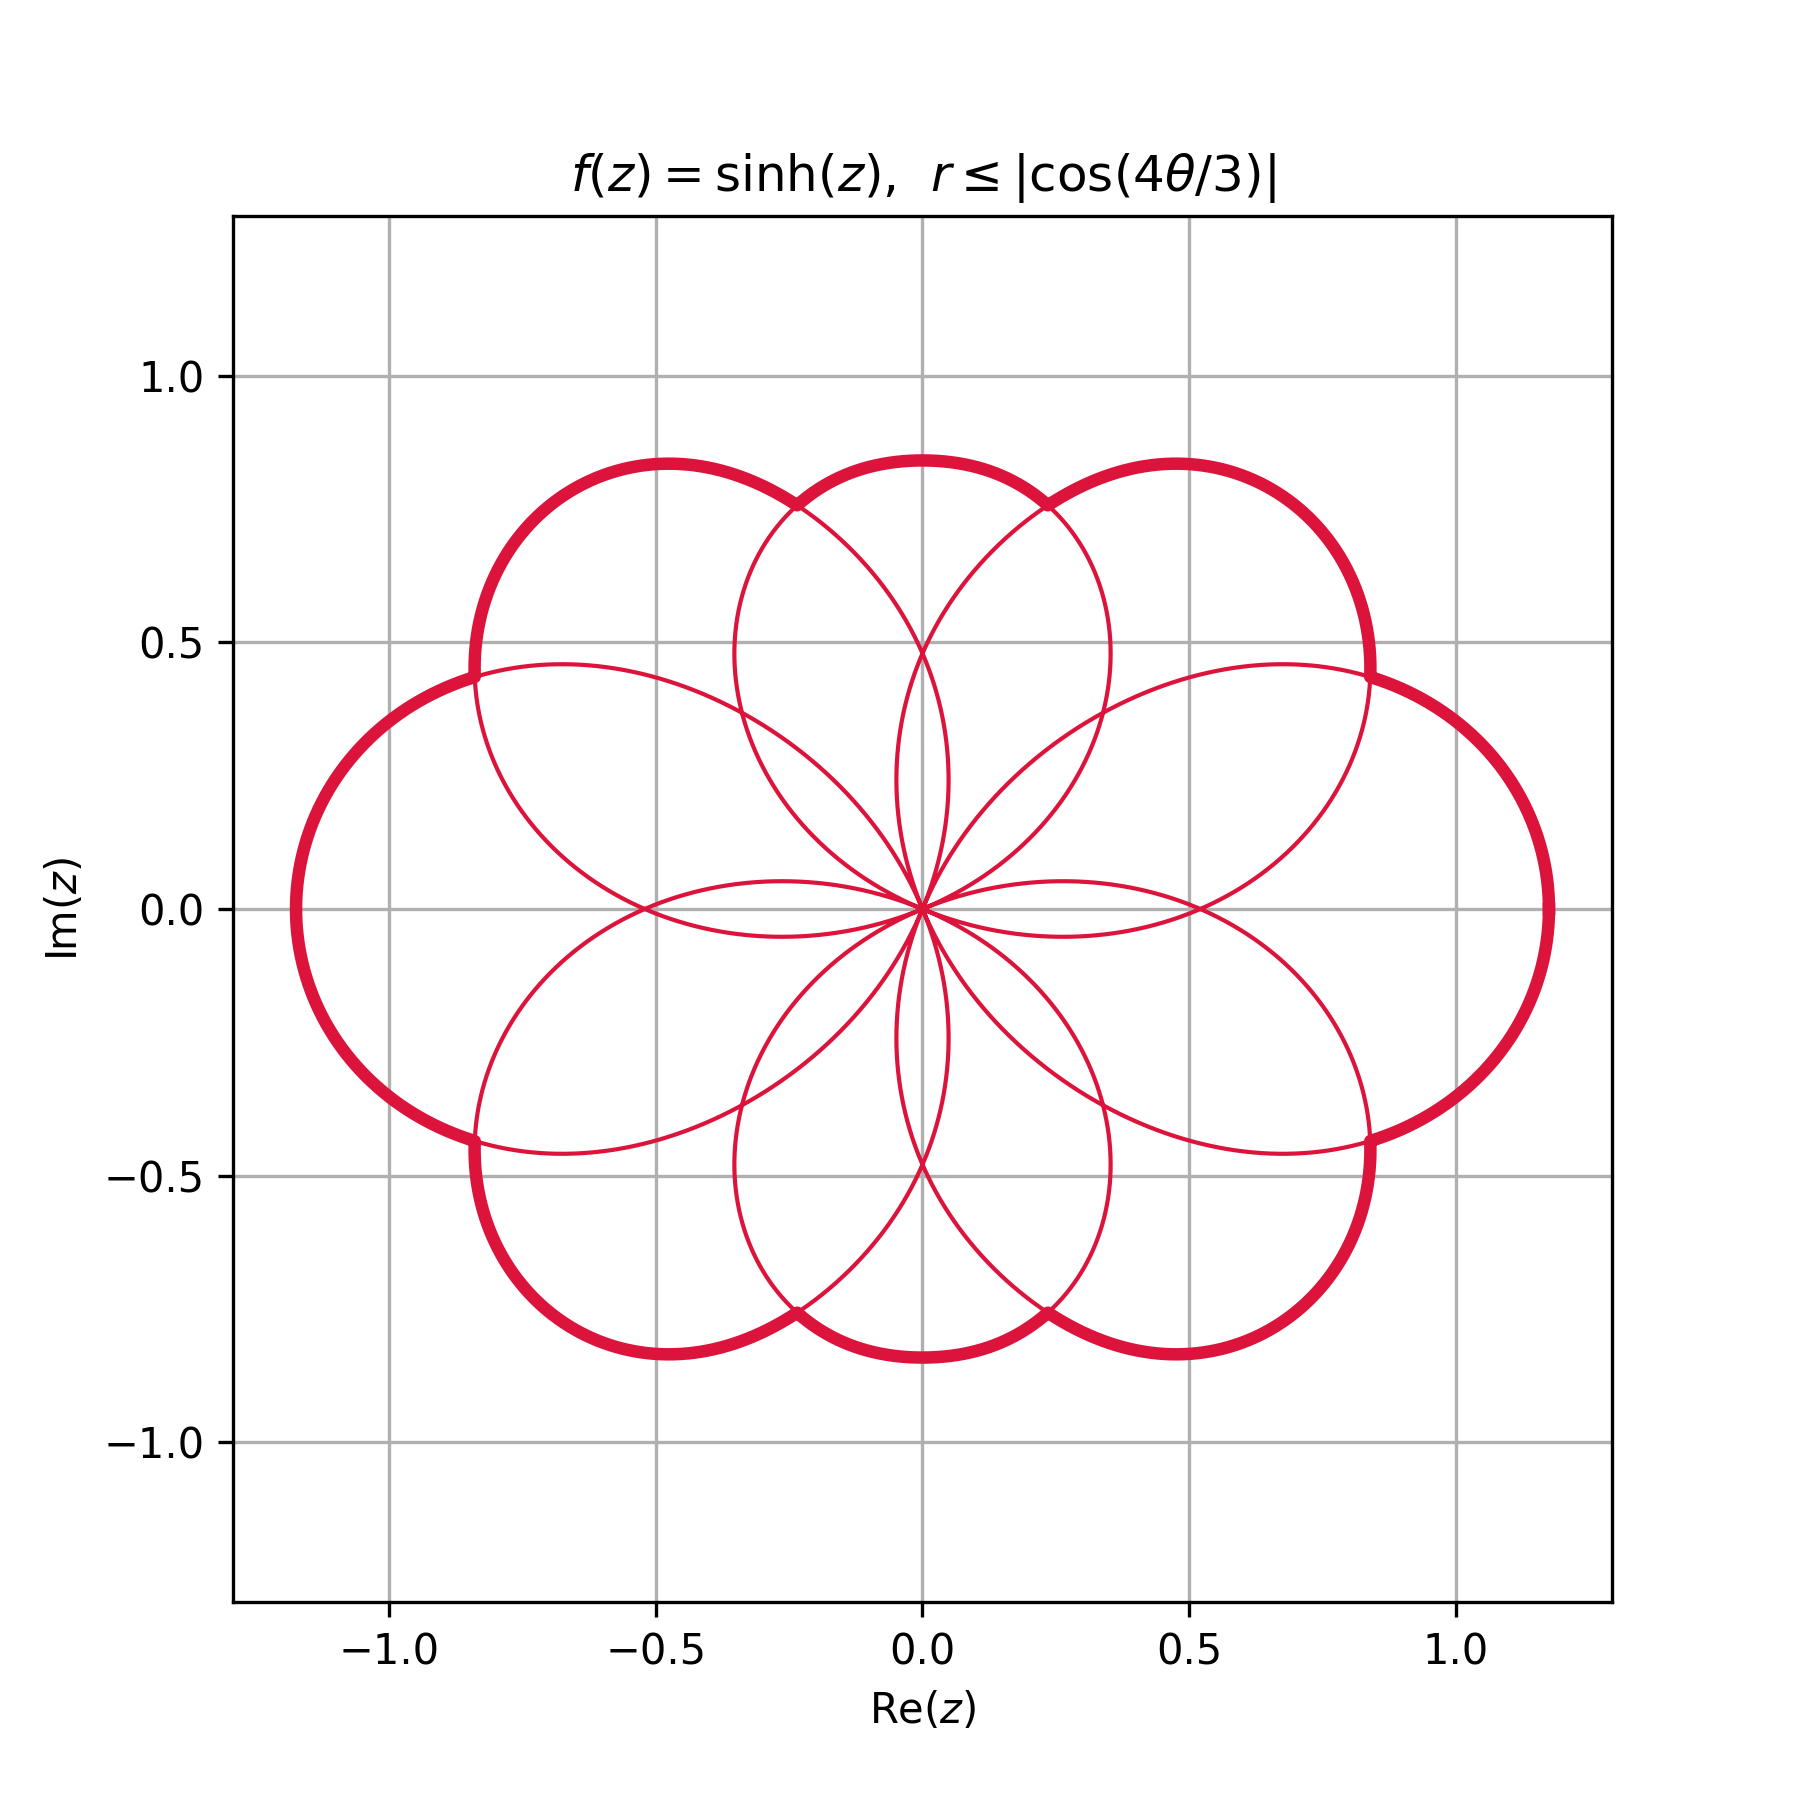
\includegraphics[width=\textwidth]{img/flower300dpi.png}
        \caption{\; Образ розы}
    \end{subfigure} \vspace*{5pt}
    \caption{ \centering Конф. отображение внутренности розы $D=\bigl\{ z\in \mathbb{C}:|z|\leq|\cos(4\arg(z)/3)|\bigr\}$ \\ функцией $f(z)=\sinh(z)$ по методу \textbf{А1.1}}
\end{figure}

\begin{displayquote}
\textbf{A1.1.} На прообразе $T$ границы исходной области выберем конечное разбиение $T_n = \{t_1,...,t_n\}$, фактически порождающее \textbf{ломанную аппроксимирующую} $\partial D$. Ломанная построенная по конформным отображениям этих точек -- то есть по множеству точек $f\bigl(g(T_n)\bigr)$ -- будет являться аппроксимацией границы $\partial D'$.
\end{displayquote} \par
Недостатком описанного метода является отсутствие какой-либо информации о том как данное конформное отображение действует внутри самой области. Именно поэтому помимо самой границы зачастую рассматривают отображение некоторой естественной координатной сетки, заданной на изначальной области (см. рис 2). Таким образом, хорошим дополнением к алгоритму \textbf{А1.1} является
\begin{displayquote}
\textbf{A1.2.} Рассмотрим некоторую \q{простую} область $S$ (как правило прямоугольник или окружность), описывающую область $D$. Введём некоторую \textbf{ортогональную координатную сетку} на $S$ и построим её конформное отображение. 
\end{displayquote}
Остаётся только заметить, что при уменьшении диаметра разбиения точность аппроксимации будет расти, а наилучший графический результат будут давать неравномерные разбиения границы, чья плотность в окрестности точки $z$ границы $\partial D$ пропорциональна $|f(z)|$. \vspace*{-0.3cm}
\begin{figure}[h!]
    \centering
    \hspace{-0.5cm}
    \begin{subfigure}{0.48\textwidth}
        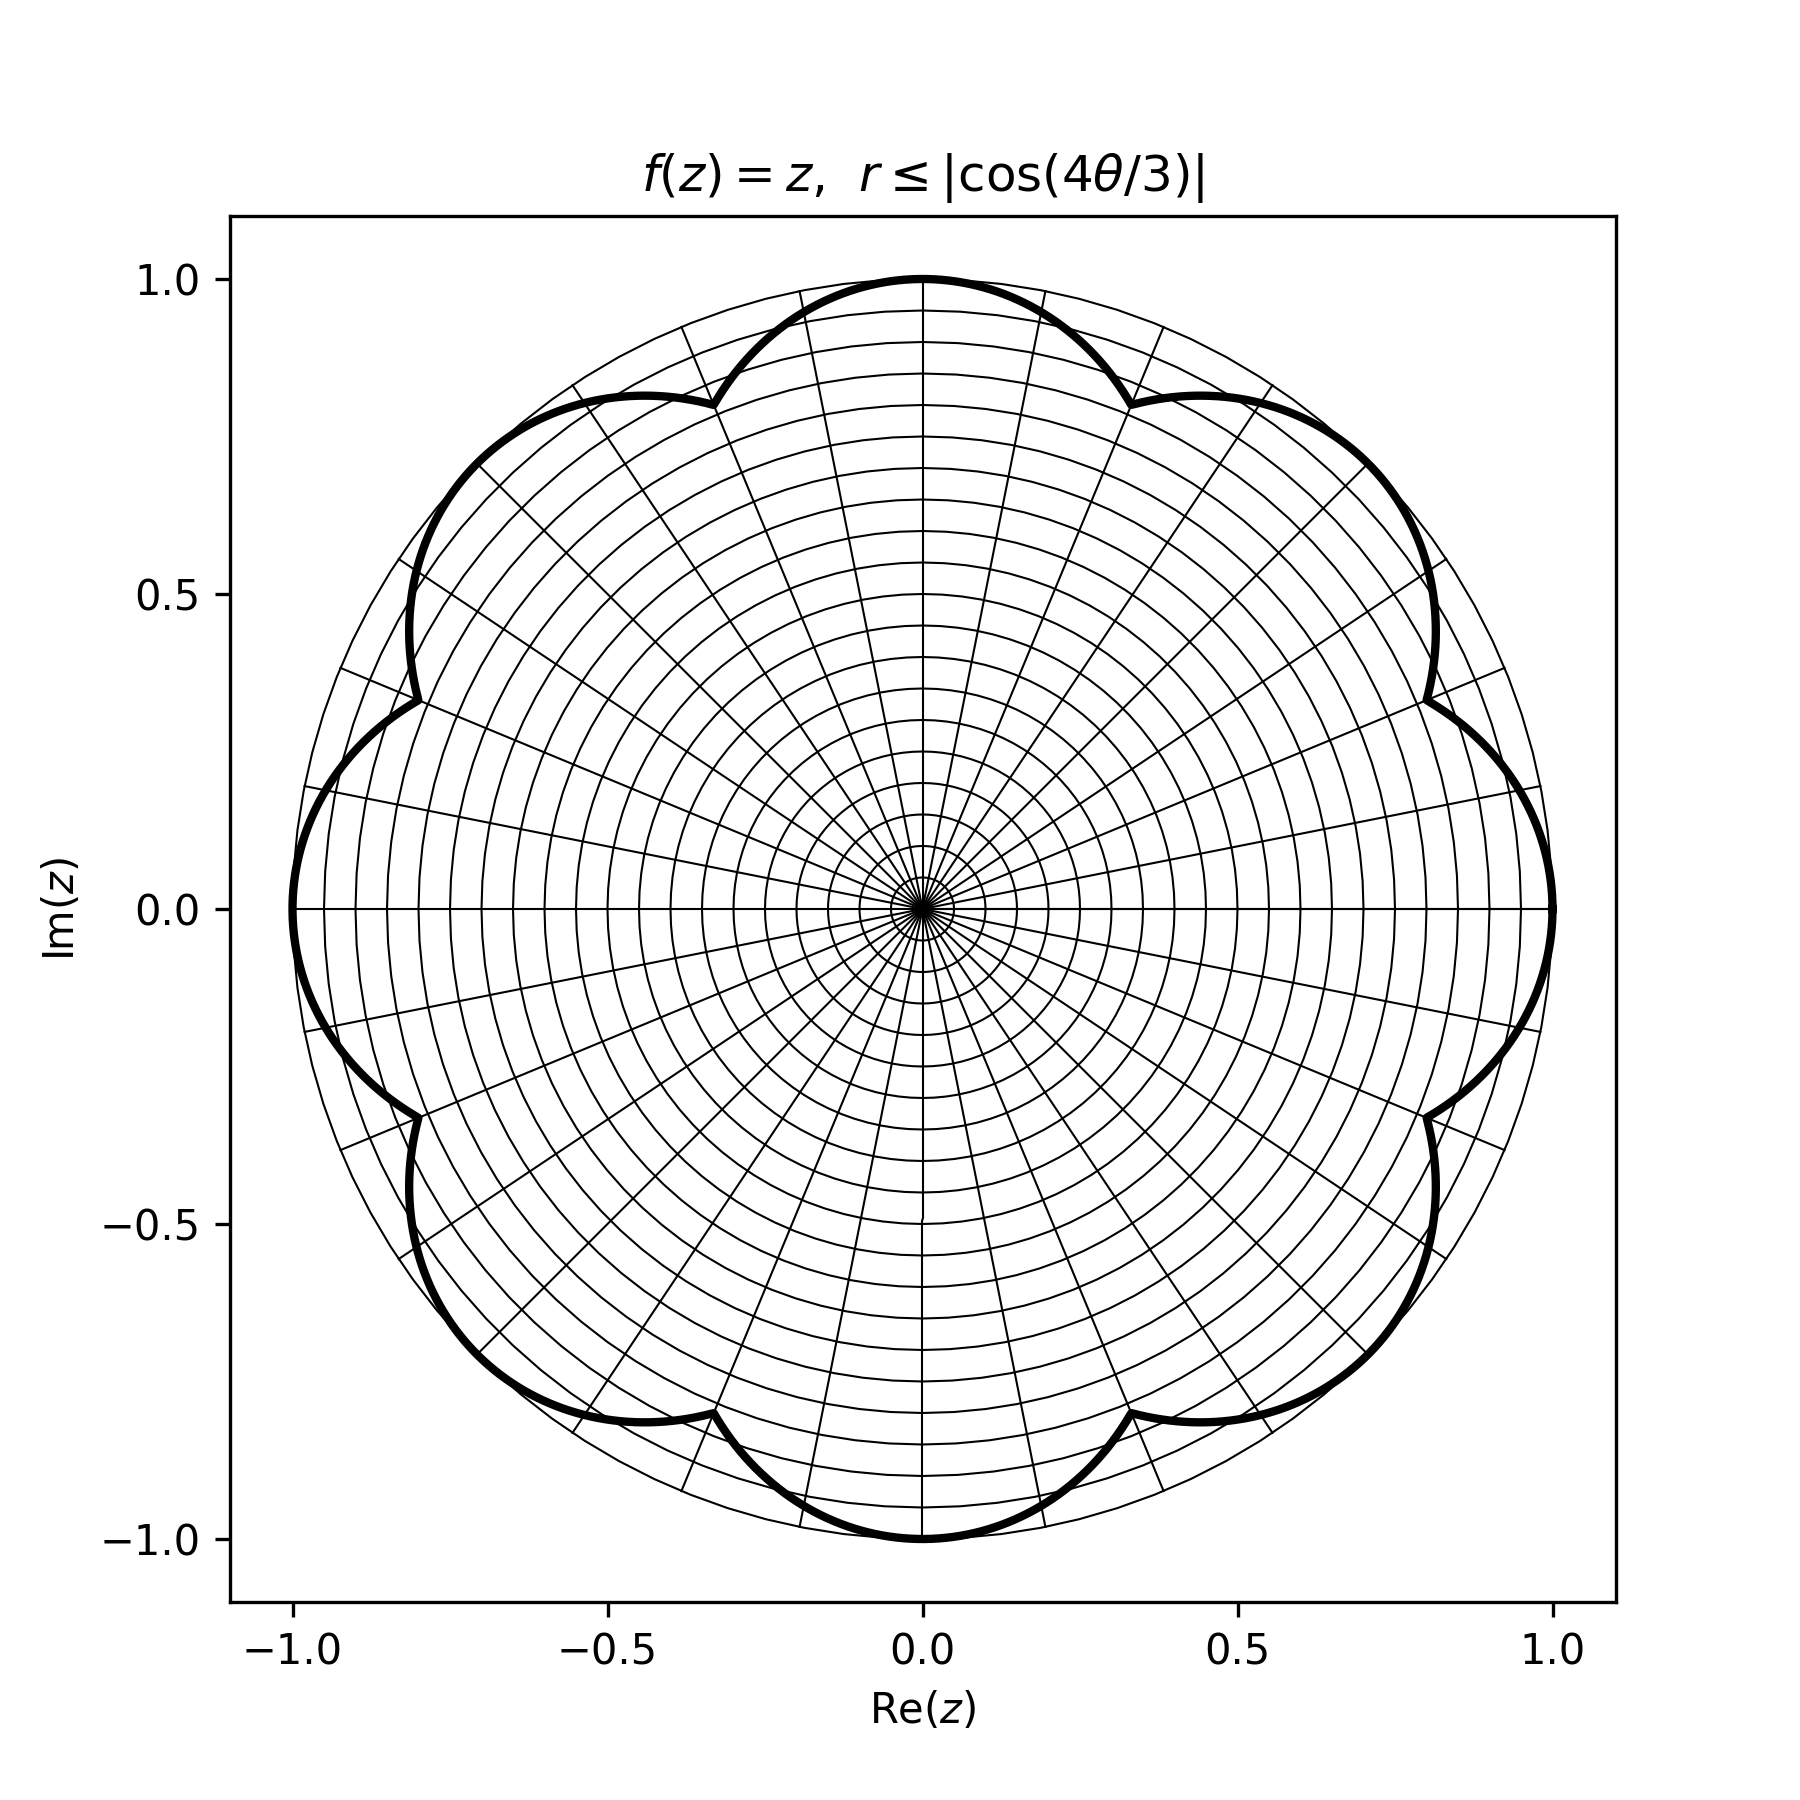
\includegraphics[width=\textwidth]{img/init_grid300dpi.png}
        \caption{\; Прообраз розы}
    \end{subfigure} \hspace{0.1cm}
    \begin{subfigure}{0.48\textwidth}
        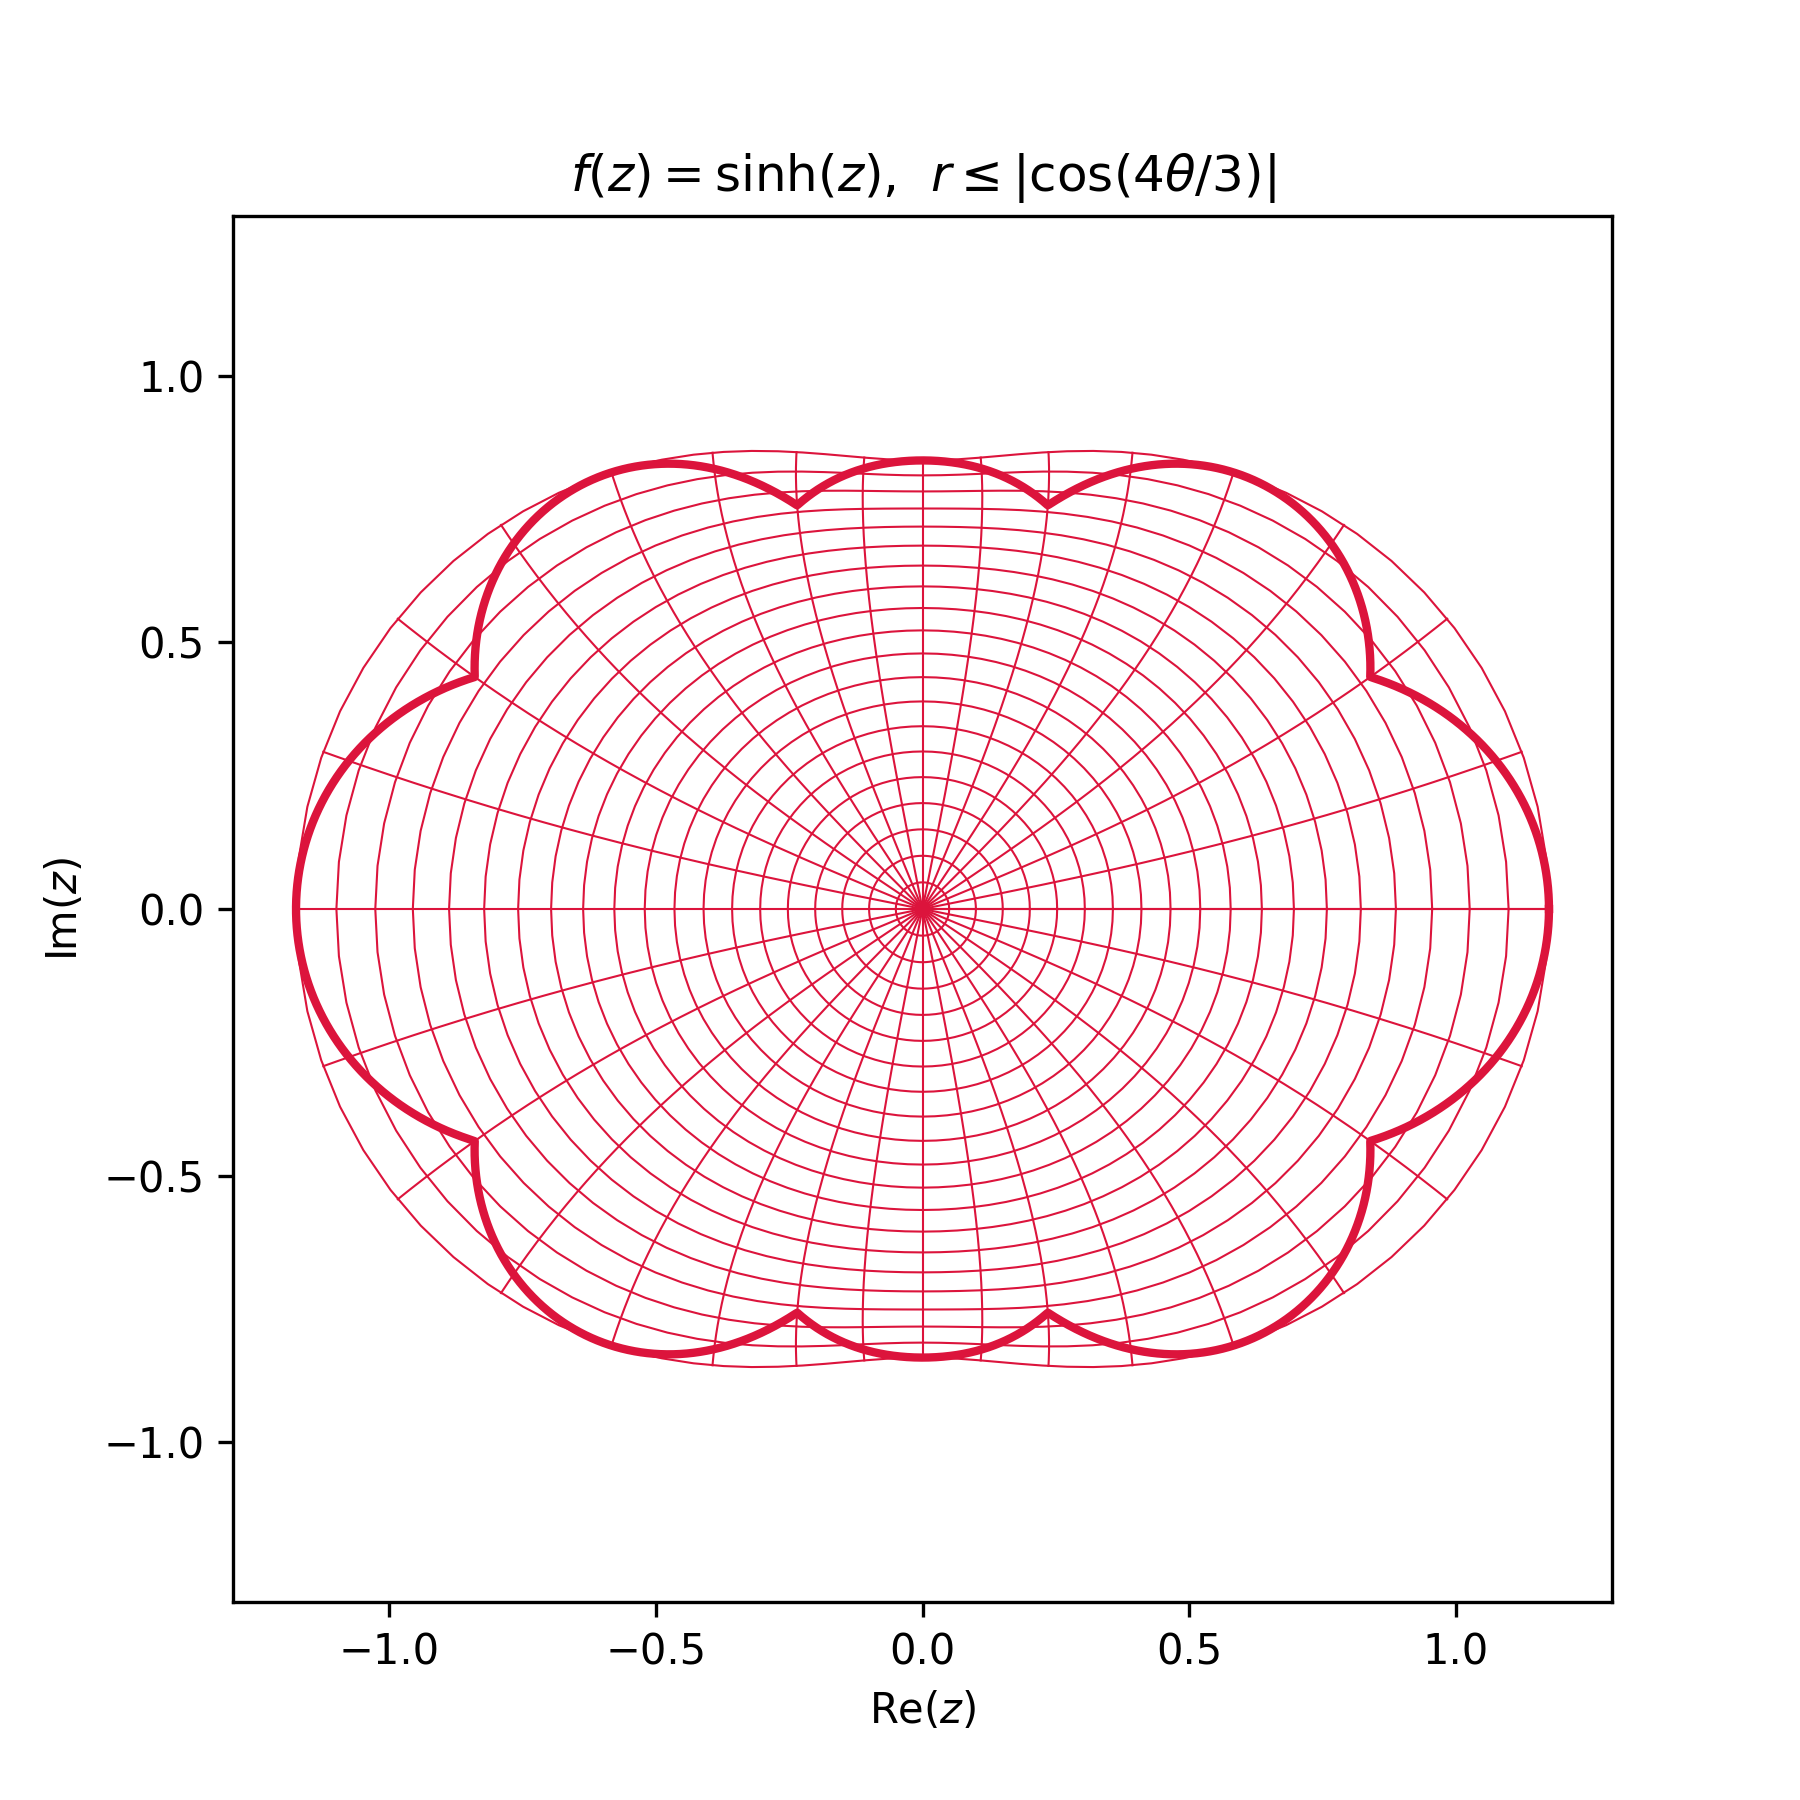
\includegraphics[width=\textwidth]{img/grid300dpi.png}
        \caption{\; Образ розы}
    \end{subfigure} \vspace*{5pt}
    \caption{ \centering Конф. отображение внутренности розы $D=\bigl\{ z\in \mathbb{C}:|z|\leq|\cos(4\arg(z)/3)|\bigr\}$ \\ функцией $f(z)=\sinh(z)$ по методу \textbf{А1.1+A1.2}}
\end{figure} \vspace*{-0.1cm}
\section{Раскраска областей}
Описанный метод аппроксимации границы $\partial D'$ хорошо работает при известной параметризации, но почти не применим при менее явных способах задания границы. Кроме того, метод \textbf{A1.2} перестаёт быть наглядными при необходимости использования очень плотных координатных сеток. Для разрешения этих трудностей можно попробовать применить метод \textbf{A2}, частично основанный на основной идее доказательства \textit{теоремы Тонелли-Фубини} в анализе.
\begin{displayquote}
\textbf{A2.} Рассмотрим некоторую \q{простую} область $S$ (прямоугольник или окружность), описывающую область $D$. Введём \textbf{конечное двумерное разбиение} на $S$, произведём \textbf{раскраску области (domain coloring)} и построим конформные отображение всех точек этого разбиения (сохраняя их цвет при изначальной раскраске), попавших внутрь области $D$. 
\end{displayquote}
В качестве \textit{раскраски конечной области} может быть использована любая градиентная палитра, но зачастую используется следующая функциональная зависимость цветовых параметров стандарта \verb_HSL_:
\begin{equation*}
H = \arg(z), \quad S = 1, \quad L = \dfrac{|z|^a}{|z|^a + 1},
\end{equation*}
которая при $a>0$ подходит и для раскраски неограниченных областей ($a=1$ в случае рис. 3) \cite{Eng}\cite{online}. \\
\textit{Замечание:} описанные методы хорошо подходят для случаев, когда $D$ и $D'$ являются ограниченными областями. В противном случае они естественно требуют довольно специфичных модификаций.
\begin{figure}[p]
    \centering
    \begin{subfigure}{0.65\textwidth}
        \includegraphics[width=\textwidth]{img/init_tight300dpi.png}
        \caption{\; Прообраз розы}
    \end{subfigure}
    \begin{subfigure}{0.65\textwidth}
    \vspace*{0.6cm}
        \includegraphics[width=\textwidth]{img/tight300dpi.png}
        \caption{\; Образ розы}
    \end{subfigure}
    \vspace*{0.25cm}
    \caption{ \centering Конф. отображение внутренности розы $D=\bigl\{ z\in \mathbb{C}:|z|\leq|\cos(4\arg(z)/3)|\bigr\}$ \\ функцией $f(z)=\sinh(z)$ по методу \textbf{A.2}}
\end{figure}
\newpage
\section{Условия вариантов и рекомендации}
\begin{task}
\textit{Численная аппроксимация решения прямой задачи конформных отображений} \\
Цель данной задачи состоит в ознакомлении с элементарными численными методами построения образов конформных отображений и использовании описанных выше методов \textbf{A1.1, A1.2} и их аналогов/вариаций для аппроксимации образа внутренности розы
\begin{equation*}
D_1 = \bigl\{ z\in\mathbb{C}: |z|\leq \alpha\cdot \max_{n\in\mathbb{Z}}|\cos\bigl(\beta\cdot (\textrm{Arg}(z) + 2n\pi)\bigr)|\, \bigr\}
\end{equation*} при конформном отображении функцией $f(z)$. Требуется:
\begin{enumerate}
\item Построить аналоги рис. 1 методом \textbf{A1} или его модификацией;
\item Создать визуализации, аналогичные рис. 2 и демонстрирующие возникающую при конформном отображении деформацию комплексной плоскости.
\end{enumerate}
\end{task} \vspace{0.1cm}
\begin{task}
\textit{Методы раскраски областей на комплексной плоскости} \\
Цель данной задачи состоит в освоении методов контекстной раскраски областей при построении графиков образа конформного отображения. Необходимо построить визуализацию образа области 
\begin{equation*}
D_2 = \bigl\{ z\in\mathbb{C}: \alpha_1\cdot \max_{n\in\mathbb{Z}}|\cos\bigl(\beta_1\cdot (\textrm{Arg}(z) + 2n\pi)\bigr)| \leq 
|z|\leq \alpha_2\cdot \max_{n\in\mathbb{Z}}|\cos\bigl(\beta_2 \cdot(\textrm{Arg}(z) + 2n\pi)\bigr)|\, \bigr\}
\end{equation*} при конформном отображении функцией $g(z)$ (методом \textbf{A2} или его аналогом), используя некоторую достаточно дескриптивную раскраску прообраза $D_2$. \\
\textit{Замечание:} функция $\textrm{Arg}: \mathbb{C}\rightarrow [0,2\pi)$ есть главное значение аргумента комплексного числа.
\end{task}
В качестве отчётности предоставляются файлы с исходным кодом и получившиеся графики.
\vspace{0.6cm}
\renewcommand*{\arraystretch}{1.8}
\begin{longtable}[c]{|c||c|c|c||c|c|c|c|c|}
\hline
\multirow{2}{*}{\textnumero} & \multicolumn{3}{c||}{Задание 1} & \multicolumn{5}{c|}{Задание 2} \\ \cline{2-9}
 & $f(z)$ & $\alpha$ & $\beta$ & $g(z)$ & $\alpha_1$ & $\beta_1$ & $\alpha_2$ & $\beta_2$ \\ \hline\hline \endhead
1  & $\sin(z/2)$ & 1.5 & 3/2 &     $(3z-1)/(3-z)$             & 0.4   & 3/5 & 1.2  & 9/7 \\ \hline
2  & $(3z-1)/(3-z)$ & 1.2 & 7/2 &  $\exp(2z)$                 & 0.2   & 2/5 & 0.8  & 3/7 \\ \hline
3  & $\exp(2z)$ & 0.8 & 2/3 &      $\textrm{arsinh}(z)$       & 0.25  & 7/4 & 0.75 & 2/7 \\ \hline
4  & $\textrm{arsinh}(z)$ & 0.75 & 5/3 &   $\tanh(z)$         & 0.2   & 1/6 & 0.5  & 3/2 \\ \hline
5  & $\tanh(z)$ & 0.5 & 7/3 &      $(4z-3)/(4-3z)$            & 0.25  & 4/5 & 1.0  & 7/2 \\ \hline
6  & $(2z-1)/(2-z)$ & 1.5 & 1/4 &  $\sin(z/2)$                & 0.25  & 1/4 & 1.5  & 2/3 \\ \hline
7  & $(4z-3)/(4-3z)$ & 1.0 & 3/4 & $\sinh(z/3)$               & 0.4   & 5/3 & 1.2  & 1/6 \\ \hline
8  & $\sinh(z/3)$ & 1.2 & 7/4 &    $(2z-1)/(2-z)$             & 0.3   & 7/3 & 1.5  & 4/5 \\ \hline
9  & $\arcsin(z)$ & 0.75 & 2/5 &   $2\exp(-z)$                & 0.3   & 3/4 & 0.9  & 1/4 \\ \hline
10 & $2\exp(-z)$ & 0.9 & 3/5 &     $(4z-1)/(4-z)$             & 0.4   & 9/7 & 2.0  & 5/3 \\ \hline
11 & $(4z-1)/(4-z)$ & 2.0 & 4/5 &  $\tan(z/4)$                & 0.4   & 3/7 & 1.6  & 7/3 \\ \hline
12 & $\tan(z/4)$ & 1.6 & 1/6 &     $\arcsin(z)$               & 0.2   & 2/7 & 0.75 & 3/4 \\ \hline
13 & $1 + \sin(3z)$ & 0.4 & 2/7 &  $(3z-2)/(3-2z)$            & 0.3   & 2/3 & 1.2  & 3/5 \\ \hline
14 & $\textrm{artanh}(z)$ & 0.5 & 3/7 &  $1 + \sin(3z)$       & 0.1   & 7/2 & 0.4  & 2/5 \\ \hline
15 & $(3z-2)/(3-2z)$ & 1.2 & 9/7 & $i\,\sin(iz/2)$            & 0.3   & 3/2 & 0.9  & 7/4 \\ \hline \newpage
16 & $i\,\sin(iz/2)$ & 0.9 & 9/7 & $(3z-i)/(3+iz)$            & 0.4   & 7/4 & 1.8  & 3/2 \\ \hline
17 & $(3z-i)/(3+iz)$ & 1.8 & 3/7 & $\exp(2iz)$                & 0.2   & 2/5 & 0.75 & 7/2 \\ \hline
18 & $\exp(2iz)$ & 0.75 & 2/7 &     $i\textrm{arsinh}(z)$     & 0.2   & 3/5 & 0.9  & 2/3 \\ \hline
19 & $i\textrm{arsinh}(z)$ & 0.9 & 1/6 & $(4z+3i)/(4-3iz)$    & 0.3   & 3/4 & 0.8  & 2/7 \\ \hline
20 & $-2i\tanh(z)$ & 0.6 & 4/5 &   $(2z-i)/(2+iz)$            & 0.5   & 7/3 & 1.75 & 3/7 \\ \hline
21 & $(2z-i)/(2+iz)$ & 1.75 & 3/5 & $\textrm{artanh}(z)$      & 0.125 & 5/3 & 0.5  & 9/7 \\ \hline
22 & $(4z+3i)/(4-3iz)$ & 0.8 & 2/5 & $-2i\tanh(z)$            & 0.1   & 1/4 & 0.6  & 3/4 \\ \hline
23 & $\sinh(iz/4)$ & 2.0 & 7/4 &   $\arcsin(iz/2)$            & 0.5   & 4/5 & 1.2  & 7/3 \\ \hline
24 & $\arcsin(iz/2)$ & 1.2 & 3/4 & $\exp(iz- i)$              & 0.2   & 1/6 & 0.75 & 5/3 \\ \hline
25 & $\exp(iz- i)$ & 0.75 & 1/4 &  $(4z+i)/(4-iz)$            & 0.4   & 2/3 & 1.0  & 1/4 \\ \hline
26 & $(4z+i)/(4-iz)$ & 1.0 & 7/3 & $\tan(iz/4)$               & 0.8   & 7/2 & 2.4  & 4/5 \\ \hline
27 & $\tan(iz/4)$ & 2.4 & 5/3 &    $i - \sinh(3z)$            & 0.1   & 3/2 & 0.3  & 1/6 \\ \hline
28 & $i - \sinh(3z)$ & 0.3 & 2/3 & $i\,\textrm{artanh}(iz)$   & 0.1   & 2/7 & 0.4  & 7/4 \\ \hline
29 & $i\,\textrm{artanh}(iz)$ & 0.4 & 7/2 & $(3z-2i)/(3+2iz)$ & 0.4   & 3/7 & 1.25 & 2/5 \\ \hline
30 & $(3z-2i)/(3+2iz)$ & 1.25 & 3/2 & $\sinh(iz/4)$           & 0.75  & 9/7 & 2.0  & 3/5 \\ \hline
\end{longtable}
\vspace*{0.1cm} \noindent
\textbf{Направления для развития:}
\begin{itemize}
\item[---] Описанные в разделе 2 методы могут быть использованы для построения графиков комплексных функций. Так, помимо традиционных графиков действительной и мнимой части, модуля и аргумента, часто используются методы визуализации, основанные на раскраске всей комплексной плоскости. Детальнее смотрите, например, \cite{Eng}\cite{online};
\item[---] Существует численные методы аппроксимации решений обратной задачи теории конформных отображений, основанные на различных видах аппроксимации функций комплексного переменного, реализующих искомое отображение. Детальнее смотрите, например, \cite{1}.
\end{itemize}

\begin{thebibliography}{99}
\RBibitem{1}
\by В. Коппенфельс, Ф. Штальман
\book Практика конформных отображений
\publ Издательство иностранной литературы
\publaddr Москва
\yr 1963

\RBibitem{2}
\by В.И. Лаврик, В.Н. Савенков
\book Справочник по конформным отображениям
\publ Издательство \q{Наукова думка}
\publaddr Киев
\yr 1970


\RBibitem{3}
\by В.И. Иванов, В.Ю. Попов
\book Конформные отображения и их приложения
\publ УРСС
\publaddr Москва
\yr 2002

\RBibitem{Shabat}
\by Б.В. Шабат
\inbook Введение в комплексный анализ
\vol 1
\publ Наука
\publaddr Москва
\yr 1976
\edition 2
\pages 228--234

\Bibitem{Eng}
\by E. Wegert
\book Visual Complex Functions
\publ Birkhäuser
\publaddr Basel
\yr 2012

\Bibitem{online}
\eprint Visualizing complex-valued functions with Matplotlib and Mayavi; Domain coloring method
\eprintinfo (visited: 2024-05-08)
\elink \href{https://notebook.community/empet/Math/DomainColoring}{https://notebook.community/empet/Math/DomainColoring}

\end{thebibliography}
\begin{center} \Large
\LaTeX
\end{center}
\end{document}